\documentclass{article}
\usepackage{amsmath}
\usepackage{amssymb}
\usepackage{graphicx}
\usepackage{hyperref}
\usepackage[version=4]{mhchem}


\begin{document}
\section*{Problem}
(2011 AIME II) In triangle \(A B C, A B=\frac{20}{11} A C\). The angle bisector of \(\angle A\) intersects \(B C\) at point \(D\), and point \(M\) is the midpoint of \(A D\). Let \(P\) be the point of the intersection of \(A C\) and \(B M\). The ratio of \(C P\) to \(P A\) can be expressed in the form \(\frac{m}{n}\), where \(m\) and \(n\) are relatively prime positive integers. Find \(m+n\).\\
\centering
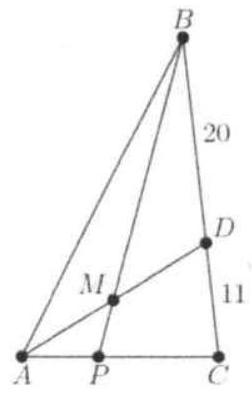
\includegraphics[width=\textwidth]{images/065(3).jpg}

\section*{Solution}
51.
Through \(D\) draw a parallel to line \(B P\) intersecting line \(A C\) at \(Q\). Then \(P Q=20 k, Q C=11 k\), and \(P A=20 k\), using the Angle Bisector Theorem and the fact that 3 or more parallel lines divide all transversals in the same proportions. Thus \(\frac{C P}{P A}=\frac{20 K+11 K}{20 K}=\frac{31}{20}\). \(m+n=31+20=51\).\\
\centering
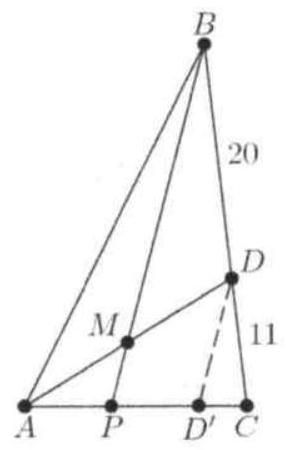
\includegraphics[width=\textwidth]{images/070.jpg}

\end{document}
